

\documentclass[12pt,a4paper]{article}\usepackage[]{graphicx}\usepackage[]{color}
%% maxwidth is the original width if it is less than linewidth
%% otherwise use linewidth (to make sure the graphics do not exceed the margin)
\makeatletter
\def\maxwidth{ %
  \ifdim\Gin@nat@width>\linewidth
    \linewidth
  \else
    \Gin@nat@width
  \fi
}
\makeatother

\definecolor{fgcolor}{rgb}{0.345, 0.345, 0.345}
\newcommand{\hlnum}[1]{\textcolor[rgb]{0.686,0.059,0.569}{#1}}%
\newcommand{\hlstr}[1]{\textcolor[rgb]{0.192,0.494,0.8}{#1}}%
\newcommand{\hlcom}[1]{\textcolor[rgb]{0.678,0.584,0.686}{\textit{#1}}}%
\newcommand{\hlopt}[1]{\textcolor[rgb]{0,0,0}{#1}}%
\newcommand{\hlstd}[1]{\textcolor[rgb]{0.345,0.345,0.345}{#1}}%
\newcommand{\hlkwa}[1]{\textcolor[rgb]{0.161,0.373,0.58}{\textbf{#1}}}%
\newcommand{\hlkwb}[1]{\textcolor[rgb]{0.69,0.353,0.396}{#1}}%
\newcommand{\hlkwc}[1]{\textcolor[rgb]{0.333,0.667,0.333}{#1}}%
\newcommand{\hlkwd}[1]{\textcolor[rgb]{0.737,0.353,0.396}{\textbf{#1}}}%
\let\hlipl\hlkwb

\usepackage{framed}
\makeatletter
\newenvironment{kframe}{%
 \def\at@end@of@kframe{}%
 \ifinner\ifhmode%
  \def\at@end@of@kframe{\end{minipage}}%
  \begin{minipage}{\columnwidth}%
 \fi\fi%
 \def\FrameCommand##1{\hskip\@totalleftmargin \hskip-\fboxsep
 \colorbox{shadecolor}{##1}\hskip-\fboxsep
     % There is no \\@totalrightmargin, so:
     \hskip-\linewidth \hskip-\@totalleftmargin \hskip\columnwidth}%
 \MakeFramed {\advance\hsize-\width
   \@totalleftmargin\z@ \linewidth\hsize
   \@setminipage}}%
 {\par\unskip\endMakeFramed%
 \at@end@of@kframe}
\makeatother

\definecolor{shadecolor}{rgb}{.97, .97, .97}
\definecolor{messagecolor}{rgb}{0, 0, 0}
\definecolor{warningcolor}{rgb}{1, 0, 1}
\definecolor{errorcolor}{rgb}{1, 0, 0}
\newenvironment{knitrout}{}{} % an empty environment to be redefined in TeX

\usepackage{alltt}
\usepackage{amsmath}
\usepackage{enumerate}
\usepackage[cm]{fullpage}
\usepackage{graphicx}
\IfFileExists{upquote.sty}{\usepackage{upquote}}{}
\begin{document}
\setlength\parindent{0cm}
%\setlength{\oddsidemargin}{0.25cm}
%\setlength{\evensidemargin}{0.25cm}
\title{\Large{\textbf{Introduction to \texttt{R}}}\\
\textit{Answers to Session 8 exercises}}
\author{Statistical Consulting Centre}
\date{2 March, 2017}
\maketitle
 
 


\section{Linear regression} 
\label{sec:lm}
\begin{enumerate}[(i)]
\item Perform a linear regression between age (explanatory variable) and nerdy score (dependent variable).
\begin{knitrout}
\definecolor{shadecolor}{rgb}{0.969, 0.969, 0.969}\color{fgcolor}\begin{kframe}
\begin{alltt}
\hlstd{linear} \hlkwb{<-} \hlkwd{lm}\hlstd{(nerdy.sc}\hlopt{~}\hlstd{age,} \hlkwc{data}\hlstd{=sports.df)}
\end{alltt}
\end{kframe}
\end{knitrout}
\item Are the estimated intercept and slope significantly different from zero?
\begin{knitrout}
\definecolor{shadecolor}{rgb}{0.969, 0.969, 0.969}\color{fgcolor}\begin{kframe}
\begin{alltt}
\hlkwd{summary}\hlstd{(linear)}
\end{alltt}
\begin{verbatim}

Call:
lm(formula = nerdy.sc ~ age, data = sports.df)

Residuals:
     Min       1Q   Median       3Q      Max 
-2.06790 -0.24615  0.02059  0.32493  1.07081 

Coefficients:
             Estimate Std. Error t value Pr(>|t|)    
(Intercept)  3.130076   0.050895  61.501   <2e-16 ***
age         -0.002391   0.000932  -2.566   0.0104 *  
---
Signif. codes:  0 '***' 0.001 '**' 0.01 '*' 0.05 '.' 0.1 ' ' 1

Residual standard error: 0.5073 on 987 degrees of freedom
  (7 observations deleted due to missingness)
Multiple R-squared:  0.006626,	Adjusted R-squared:  0.00562 
F-statistic: 6.584 on 1 and 987 DF,  p-value: 0.01044
\end{verbatim}
\end{kframe}
\end{knitrout}
\item Examine the residuals of the fitted linear model.
\begin{knitrout}
\definecolor{shadecolor}{rgb}{0.969, 0.969, 0.969}\color{fgcolor}\begin{kframe}
\begin{alltt}
\hlkwd{plot}\hlstd{(}\hlkwd{residuals}\hlstd{(linear))}
\end{alltt}
\end{kframe}

{\centering 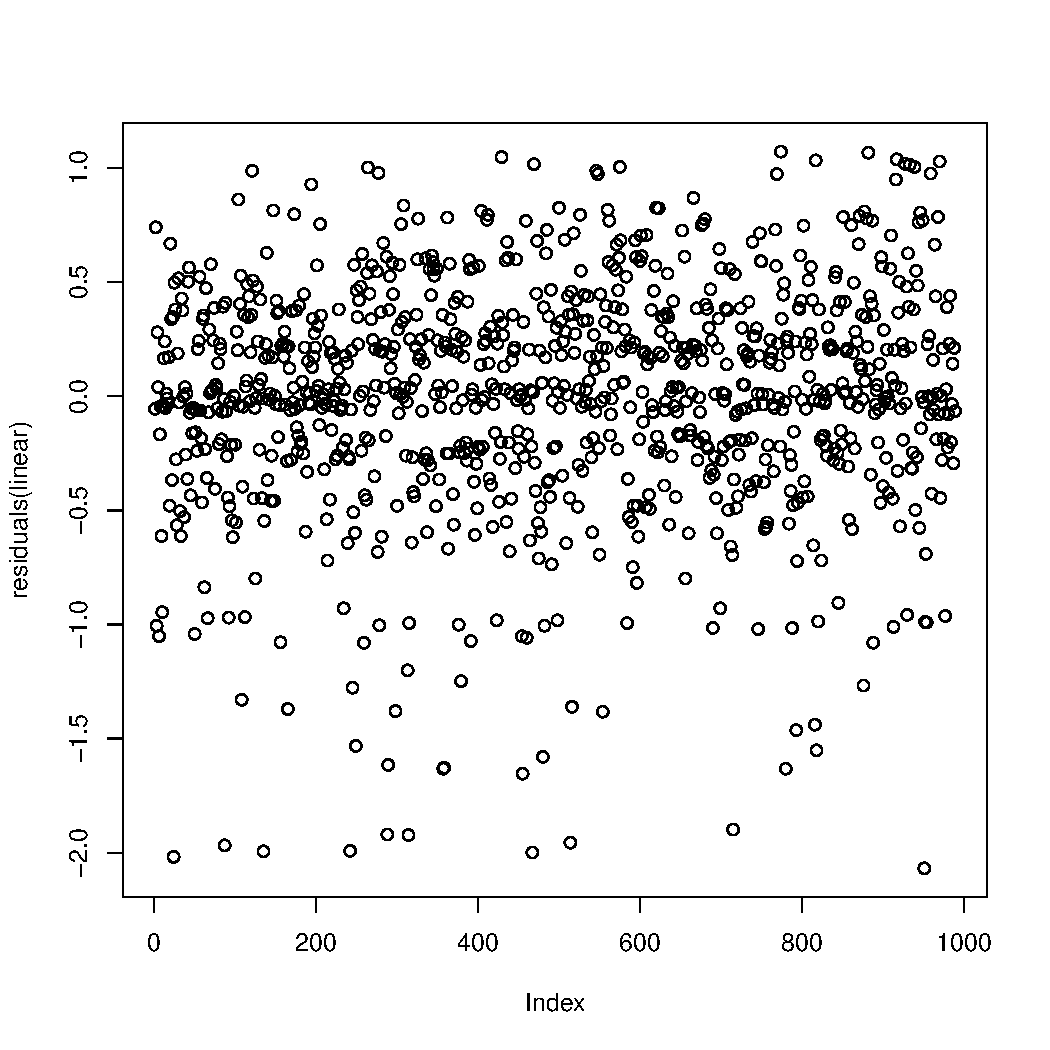
\includegraphics[width=0.6\textwidth]{figure/unnamed-chunk-4-1} 

}


\begin{kframe}\begin{alltt}
\hlkwd{qqnorm}\hlstd{(}\hlkwd{residuals}\hlstd{(linear))}
\hlkwd{qqline}\hlstd{(}\hlkwd{residuals}\hlstd{(linear),} \hlkwc{lwd} \hlstd{=} \hlnum{2}\hlstd{,} \hlkwc{col} \hlstd{=} \hlnum{2}\hlstd{)}
\end{alltt}
\end{kframe}

{\centering 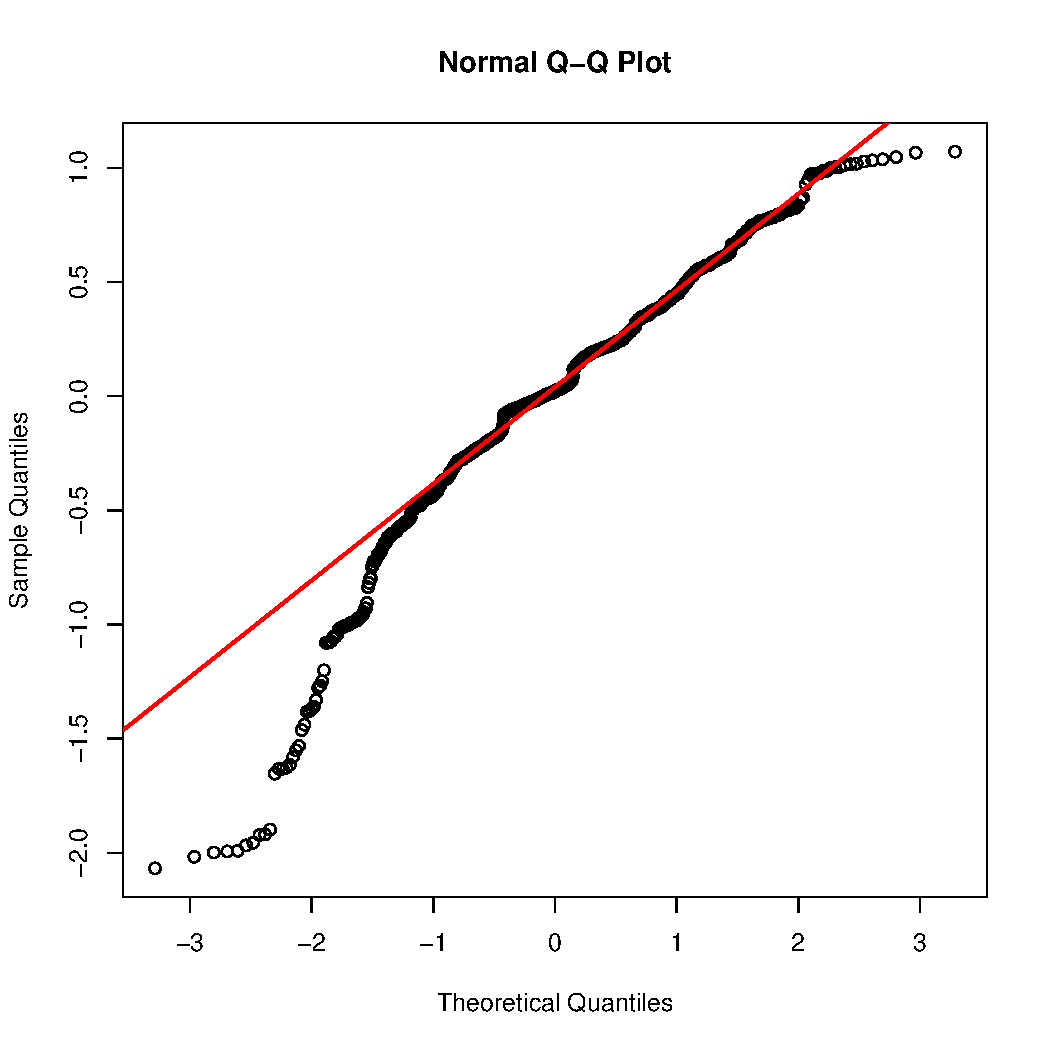
\includegraphics[width=0.6\textwidth]{figure/unnamed-chunk-4-2} 

}



\end{knitrout}
\item Add the fitted line to the scatterplot of nerdy score against age.
\begin{knitrout}
\definecolor{shadecolor}{rgb}{0.969, 0.969, 0.969}\color{fgcolor}\begin{kframe}
\begin{alltt}
\hlstd{estimated.intercept} \hlkwb{<-} \hlkwd{coef}\hlstd{(linear)[}\hlnum{1}\hlstd{]}
\hlstd{estimated.slope} \hlkwb{<-} \hlkwd{coef}\hlstd{(linear)[}\hlnum{2}\hlstd{]}
\hlkwd{with}\hlstd{(sports.df,} \hlkwd{plot}\hlstd{(age, nerdy.sc),} \hlkwc{xlab} \hlstd{=} \hlstr{"Age"}\hlstd{,} \hlkwc{ylab} \hlstd{=} \hlstr{"Nerdy score"}\hlstd{)}
\hlkwd{abline}\hlstd{(}\hlkwc{a} \hlstd{= estimated.intercept,} \hlkwc{b} \hlstd{= estimated.slope,} \hlkwc{lwd} \hlstd{=} \hlnum{2}\hlstd{,} \hlkwc{col} \hlstd{=} \hlnum{2}\hlstd{)}
\end{alltt}
\end{kframe}

{\centering 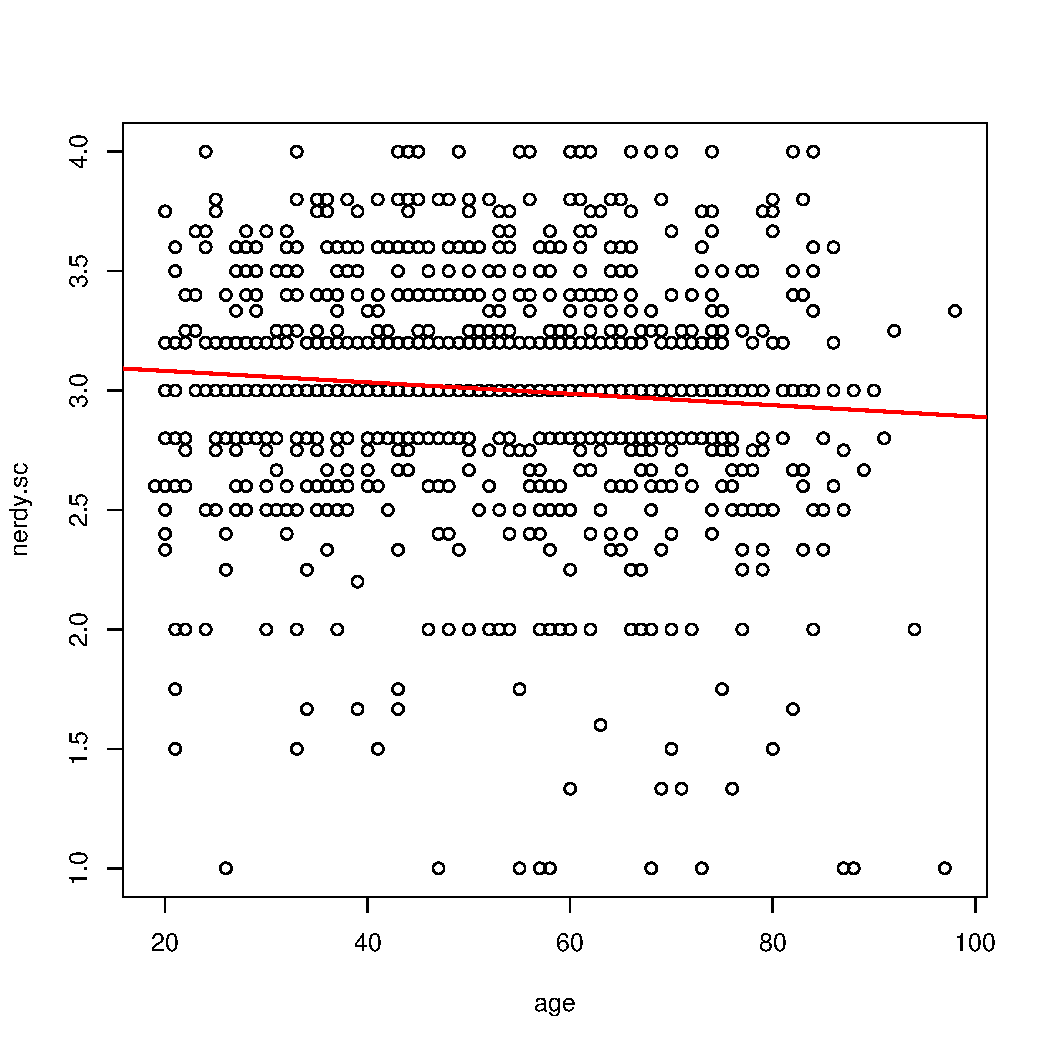
\includegraphics[width=0.6\textwidth]{figure/unnamed-chunk-5-1} 

}



\end{knitrout}
\item What conclusions can you draw? Do you think age and nerdy score are linearly correlated?
\end{enumerate}


\section{Logistic Regression} 
\label{sec:log}
\begin{enumerate}[(i)]

\subsection{Continuous explanatory variable}

\item Suppose we want to model the probability of being male, i.e., \texttt{gender = Male}. First, ensure that \texttt{gender} is a variable with a correct type. 
\begin{knitrout}
\definecolor{shadecolor}{rgb}{0.969, 0.969, 0.969}\color{fgcolor}\begin{kframe}
\begin{alltt}
\hlcom{# Check gender}
\hlkwd{class}\hlstd{(sports.df}\hlopt{$}\hlstd{gender)}
\end{alltt}
\begin{verbatim}
[1] "character"
\end{verbatim}
\begin{alltt}
\hlkwd{table}\hlstd{(sports.df}\hlopt{$}\hlstd{gender)}
\end{alltt}
\begin{verbatim}

Female   Male 
   535    461 
\end{verbatim}
\begin{alltt}
\hlstd{sports.df}\hlopt{$}\hlstd{gender} \hlkwb{<-} \hlkwd{ifelse}\hlstd{(sports.df}\hlopt{$}\hlstd{gender} \hlopt{==} \hlstr{"Male"}\hlstd{,} \hlnum{1}\hlstd{,} \hlnum{0}\hlstd{)}
\end{alltt}
\end{kframe}
\end{knitrout}
\item Fit a logistic model with \texttt{gender} as the response variable and \texttt{nerdy.sc} as the explanatory variable.
\begin{knitrout}
\definecolor{shadecolor}{rgb}{0.969, 0.969, 0.969}\color{fgcolor}\begin{kframe}
\begin{alltt}
\hlstd{myglm} \hlkwb{<-} \hlkwd{with}\hlstd{(sports.df,} \hlkwd{glm}\hlstd{(gender}\hlopt{~}\hlstd{nerdy.sc,} \hlkwc{family} \hlstd{= binomial))}
\end{alltt}
\end{kframe}
\end{knitrout}
\item Perform an analysis of deviance to determine the overall significance of \texttt{nerdy.sc}.
\begin{knitrout}
\definecolor{shadecolor}{rgb}{0.969, 0.969, 0.969}\color{fgcolor}\begin{kframe}
\begin{alltt}
\hlkwd{anova}\hlstd{(myglm,} \hlkwc{test} \hlstd{=} \hlstr{"Chisq"}\hlstd{)}
\end{alltt}
\begin{verbatim}
Analysis of Deviance Table

Model: binomial, link: logit

Response: gender

Terms added sequentially (first to last)


         Df Deviance Resid. Df Resid. Dev  Pr(>Chi)    
NULL                       988     1365.0              
nerdy.sc  1   14.677       987     1350.4 0.0001276 ***
---
Signif. codes:  0 '***' 0.001 '**' 0.01 '*' 0.05 '.' 0.1 ' ' 1
\end{verbatim}
\end{kframe}
\end{knitrout}
\item Calculate the estimated slope of the logistic regression. What can you conclude about the slope?
\begin{knitrout}
\definecolor{shadecolor}{rgb}{0.969, 0.969, 0.969}\color{fgcolor}\begin{kframe}
\begin{alltt}
\hlkwd{summary}\hlstd{(myglm)}
\end{alltt}
\begin{verbatim}

Call:
glm(formula = gender ~ nerdy.sc, family = binomial)

Deviance Residuals: 
    Min       1Q   Median       3Q      Max  
-1.3205  -1.1092  -0.9144   1.2047   1.6877  

Coefficients:
            Estimate Std. Error z value Pr(>|z|)    
(Intercept)  -1.6417     0.4026  -4.078 4.55e-05 ***
nerdy.sc      0.4930     0.1315   3.749 0.000177 ***
---
Signif. codes:  0 '***' 0.001 '**' 0.01 '*' 0.05 '.' 0.1 ' ' 1

(Dispersion parameter for binomial family taken to be 1)

    Null deviance: 1365.0  on 988  degrees of freedom
Residual deviance: 1350.4  on 987  degrees of freedom
  (7 observations deleted due to missingness)
AIC: 1354.4

Number of Fisher Scoring iterations: 4
\end{verbatim}
\end{kframe}
\end{knitrout}
\end{enumerate}

\subsection{Categorical explanatory variable}
\begin{enumerate}[(i)]
\item We now want to model the probability of living with a partner given age group. \texttt{partner} is already of type \texttt{factor}. Now, generate a one-way table of \texttt{partner} to examine its contents. %Notice that there are only \texttt{Yes} and \texttt{No} cases remaining.
\begin{knitrout}
\definecolor{shadecolor}{rgb}{0.969, 0.969, 0.969}\color{fgcolor}\begin{kframe}
\begin{alltt}
\hlkwd{table}\hlstd{(sports.df}\hlopt{$}\hlstd{partner)}
\end{alltt}
\begin{verbatim}

 No Yes 
122 229 
\end{verbatim}
\end{kframe}
\end{knitrout}
\item Set a response variable with \texttt{partner} = \texttt{Yes}.
\begin{knitrout}
\definecolor{shadecolor}{rgb}{0.969, 0.969, 0.969}\color{fgcolor}\begin{kframe}
\begin{alltt}
\hlstd{sports.df}\hlopt{$}\hlstd{partner} \hlkwb{<-} \hlkwd{ifelse}\hlstd{(sports.df}\hlopt{$}\hlstd{partner} \hlopt{==} \hlstr{"Yes"}\hlstd{,} \hlnum{1}\hlstd{,} \hlnum{0}\hlstd{)}
\end{alltt}
\end{kframe}
\end{knitrout}
\item Once again geenerate the one-way frequency table of \texttt{partner}.
\begin{knitrout}
\definecolor{shadecolor}{rgb}{0.969, 0.969, 0.969}\color{fgcolor}\begin{kframe}
\begin{alltt}
\hlkwd{table}\hlstd{(sports.df}\hlopt{$}\hlstd{partner)}
\end{alltt}
\begin{verbatim}

  0   1 
122 229 
\end{verbatim}
\end{kframe}
\end{knitrout}
\item Fit a logistic model with \texttt{partner} as the response variable and \texttt{age.group} as the explanatory variable.
\begin{knitrout}
\definecolor{shadecolor}{rgb}{0.969, 0.969, 0.969}\color{fgcolor}\begin{kframe}
\begin{alltt}
\hlstd{myglm2} \hlkwb{<-} \hlkwd{with}\hlstd{(sports.df,} \hlkwd{glm}\hlstd{(partner}\hlopt{~}\hlstd{age.group,} \hlkwc{family} \hlstd{= binomial))}
\end{alltt}
\end{kframe}
\end{knitrout}
\item Is \texttt{age.group} a significant predictor of whether or not an individual in particular age group has a partner?
\begin{knitrout}
\definecolor{shadecolor}{rgb}{0.969, 0.969, 0.969}\color{fgcolor}\begin{kframe}
\begin{alltt}
\hlkwd{anova}\hlstd{(myglm2,} \hlkwc{test} \hlstd{=} \hlstr{"Chisq"}\hlstd{)}
\end{alltt}
\begin{verbatim}
Analysis of Deviance Table

Model: binomial, link: logit

Response: partner

Terms added sequentially (first to last)


          Df Deviance Resid. Df Resid. Dev Pr(>Chi)
NULL                        350     453.45         
age.group  2  0.19833       348     453.25   0.9056
\end{verbatim}
\end{kframe}
\end{knitrout}
\item[] Not at the 5\% level of significance since $p$ = 0.91.
\item Generate a two-way frequency table of \texttt{partner} against \texttt{age.group}. 
\begin{knitrout}
\definecolor{shadecolor}{rgb}{0.969, 0.969, 0.969}\color{fgcolor}\begin{kframe}
\begin{alltt}
\hlstd{twoway.tab} \hlkwb{<-} \hlkwd{with}\hlstd{(sports.df,} \hlkwd{table}\hlstd{(partner, age.group))}
\hlstd{twoway.tab}
\end{alltt}
\begin{verbatim}
       age.group
partner Under 40 41 to 60 Over 61
      0       54       36      32
      1       96       69      64
\end{verbatim}
\end{kframe}
\end{knitrout}
\item Convert these frequencies to percentages of age group total. Does this table agree with your earlier conclusion?
\begin{knitrout}
\definecolor{shadecolor}{rgb}{0.969, 0.969, 0.969}\color{fgcolor}\begin{kframe}
\begin{alltt}
\hlkwd{round}\hlstd{(}\hlnum{100}\hlopt{*}\hlkwd{prop.table}\hlstd{(twoway.tab,} \hlnum{2}\hlstd{),} \hlnum{1}\hlstd{)}
\end{alltt}
\begin{verbatim}
       age.group
partner Under 40 41 to 60 Over 61
      0     36.0     34.3    33.3
      1     64.0     65.7    66.7
\end{verbatim}
\end{kframe}
\end{knitrout}
\item[] Yes, since the percentages of \texttt{Yes} and \texttt{No} are approximately the same across age groups.
\end{enumerate}


\end{document}
